\section*{Goal}
The goal of this lab course was to get to know and learn how to set up Diode Lasers.
With the installed diode laser the fluorescence of Rubidium got analysed.
\section{Theory}
\label{sec:theory}
The theoretical background for Lasers and especially diode lasers needs to be understood to properly work with the setup.
In this chapter everything important for the lab course is explained.
\subsection{Lasers}
Laser (Light Amplification by Stimulated Emission of Radiation) is a form of Light emission which is frequently used in the industry and for research.
Light emitted from a Laser is coherent in time (all photons have the same phase) and space (the photons travel parallel in the same direction).
The Laser-light consists of photons with the same wavelength (monochromatic) and therefore the same energy, the photons also have the same linear polarization.
To produce the light a Laser consists out of three major parts: The active medium, the energy pump and the Resonator.

The active medium determines the wavelength of the photons because they are generated by the electrons relaxing over the band gap of the material.
To create laser light a population inversion has to be created with the different energy levels in the active medium.
If we assume three energy levels in the active medium with the first level $E_1$ having the lowest energy and the third level having the highest energy.
To create population inversion in the medium, the second level $E_2$ has to have more electrons than the first (lowest) level.
The relaxation from the third to the second level $E_2$ has to be a faster transition than the transition from the second energy level to the first level $E_1$ (ground state).
To provide enough electrons in the higher level a energy pump has to be used to excite electrons from the ground state $E_1$ to the third energy level.

To relax from the second level $E_2$ to the ground state $E_1$ the electrons can either spontaneously relax and emit the corresponding photon or can be stimulated by an incoming photon to relax and therefore emit a second photon with the same properties (Orientation, Frequency, Phase and Polarization).
This stimulated emission is the main source for the photons of the laser.
The simulated emission and the spontaneous emission are shown in figure \ref{fig:emission}.

\begin{figure}
    \center
    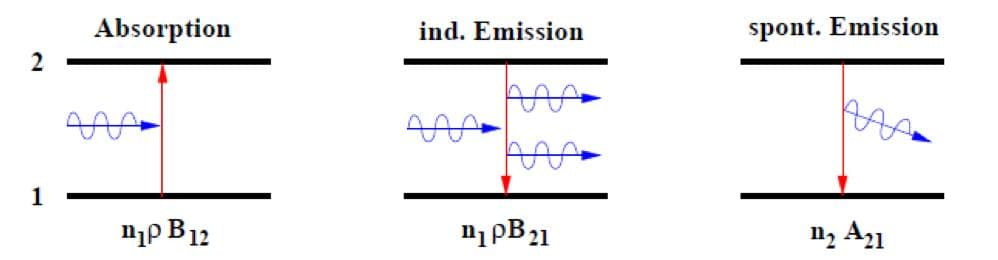
\includegraphics[width=0.8\textwidth]{bilder/emission.jpg}
    \caption{Absorption and emission in the active medium are shown for a two state system. \cite{anleitungHeNe}}
    \label{fig:emission}
\end{figure}

\subsection{Diode}
In this experiment a pn-junction diode is used.
A pn-junction diode is a part of a electrical 